\section{Pianificazione}

Al fine della pianificazione si è deciso di suddividere il progetto in cinque macro-periodo distinti:
\begin{itemize}
\item \textbf{\AR{}:} periodo di analisi iniziale;
\item \textbf{\AD{}:} periodo di analisi successiva all'accettazione della proposta;
\item \textbf{\PA{}}.
\item \textbf{\PD{} e \Cod{}}.
\item \textbf{\VV{}}.
\end{itemize}
Ogni macro-periodo è stata poi suddivisa in sotto-attività, ad ognuna delle quali sono assegnate una o più risorse. Le attività sono rappresentate attraverso diagrammi di \glossario{Gantt}. Nei diagrammi sono presenti anche le \glossario{milestone}, a rappresentare la conclusione dell'attività coincidente con la consegna dei documenti. \\
Per il glossario non è stata prevista alcuna ripartizione delle ore tra i componenti del gruppo per la redazione in quanto viene redatto contemporaneamente alla stesura degli altri documenti ogni qualvolta un termine necessiti di una spiegazione.

\subsection{\AR{}}
\textbf{Periodo:} da 10-12-2016 a 11-01-2017. \\
Tale periodo inizia in corrispondenza della data di scadenza per la formazione dei gruppi e termina con la data di consegna dei documenti per la \RR{}. Nel periodo di \AR{} vengono analizzati i requisiti derivanti dal capitolato e scelti gli strumenti, proposti direttamente dal capitolato stesso o no, che favoriscono lo sviluppo del progetto. I documenti di maggior impatto sono: \textit{Norme di progetto}, \textit{Studio di fattibilità}, \textit{Analisi dei requisiti}, \textit{Piano di qualifica}, \textit{Piano di progetto}, \textit{Glossario} e \textit{Lettera di presentazione}.
Nel periodo di Analisi i ruoli maggiormente coinvolti sono \Analista{}, \Responsabile{}, \Amministratore{} e \Verificatore{}.

\subsubsection{Gantt attività}
\begin{figure}[H]
\centering
\scalebox{0.3}{\includegraphics{gantt/Gantt_RR.png}}
\caption{Diagramma di Gantt, periodo di \AR{}}
\end{figure}

\subsubsection{Ripartizione ore}
\bgroup
\egroup
  
\subsection{\AD{}}
\textbf{Periodo:} da 25-01-2017 a 28-01-2017. \\
Tale periodo inizia in corrispondenza della revisione dei requisiti. Il periodo di \AD{} riguarda un incremento e correzione dei requisiti e dei documenti stilati durante il periodo di \AR{}: \textit{Norme di progetto}, \textit{Analisi dei requisiti}, \textit{Piano di qualifica}, \textit{Piano di progetto} e \textit{Glossario}.
Nel periodo di \AD{} i ruoli maggiormente coinvolti sono \Analista{}, \Responsabile{}, \Amministratore{} e \Verificatore{}.

\subsubsection{Gantt attività}
\begin{figure}[H]
	\centering
	\scalebox{0.3}{\includegraphics{gantt/Gantt_AD.png}}
	\caption{Diagramma di Gantt, periodo di \AD{}}
\end{figure}

\subsubsection{Ripartizione ore}
\bgroup
\egroup

\subsection{\PA{}}
\textbf{Periodo:} da 29-01-2017 a 06-03-2017.\\
Tale periodo inizia dopo il periodo di \AD{}. Il periodo di \textbf{Progettazione architetturale} riguarda lo sviluppo dell'architettura del sistema da realizzare, viene approfondita la struttura basilare del sistema e studiate le tecnologie che la compongono. I documenti che vengono incrementati in questo periodo sono: \textit{Specifica Tecnica}, accompagnata da: \textit{Norme di progetto}, \textit{Piano di qualifica} e \textit{Glossario}.
Nel periodo di \PA{} i ruoli maggiormente coinvolti sono \Progettista{}, \Responsabile{}, \Amministratore{}, \Analista{} e \Verificatore{}.
\subsubsection{Gantt attività}
\begin{figure}[H]
	\centering
	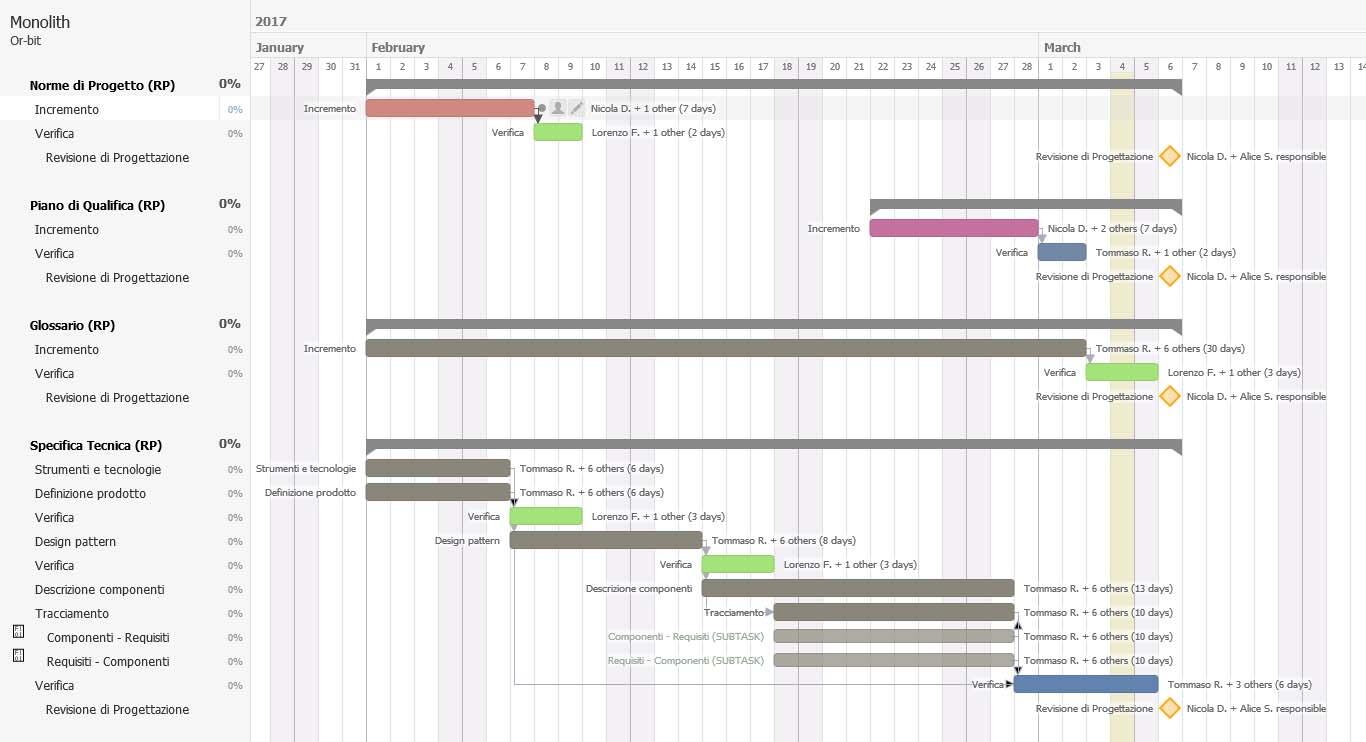
\includegraphics[width=15cm]{gantt/Gantt_RP2.png}
	\caption{Diagramma di Gantt, periodo di \PA{}}
\end{figure}

\subsubsection{Ripartizione ore}
\bgroup
\egroup

\subsection{\PD{} e \Cod{}}
\textbf{Periodo:} da 14-03-2017 a 11-04-2017. \\
Il periodo di \PD{} e \Cod{} viene utilizzato per lo sviluppo del sistema nell'ambiente scelto durante i periodi precedenti, riguarda inoltre un incremento e correzione dei documenti finora stilati e lo sviluppo del sistema da realizzare.
Nel periodo di \PD{} e \Cod{} i ruoli maggiormente coinvolti sono \Programmatore{}, \Progettista{}, \Analista{}, \Responsabile{}, \Amministratore{} e \Verificatore{}.
\subsubsection{Gantt attività}
\begin{figure}[H]
	\centering
	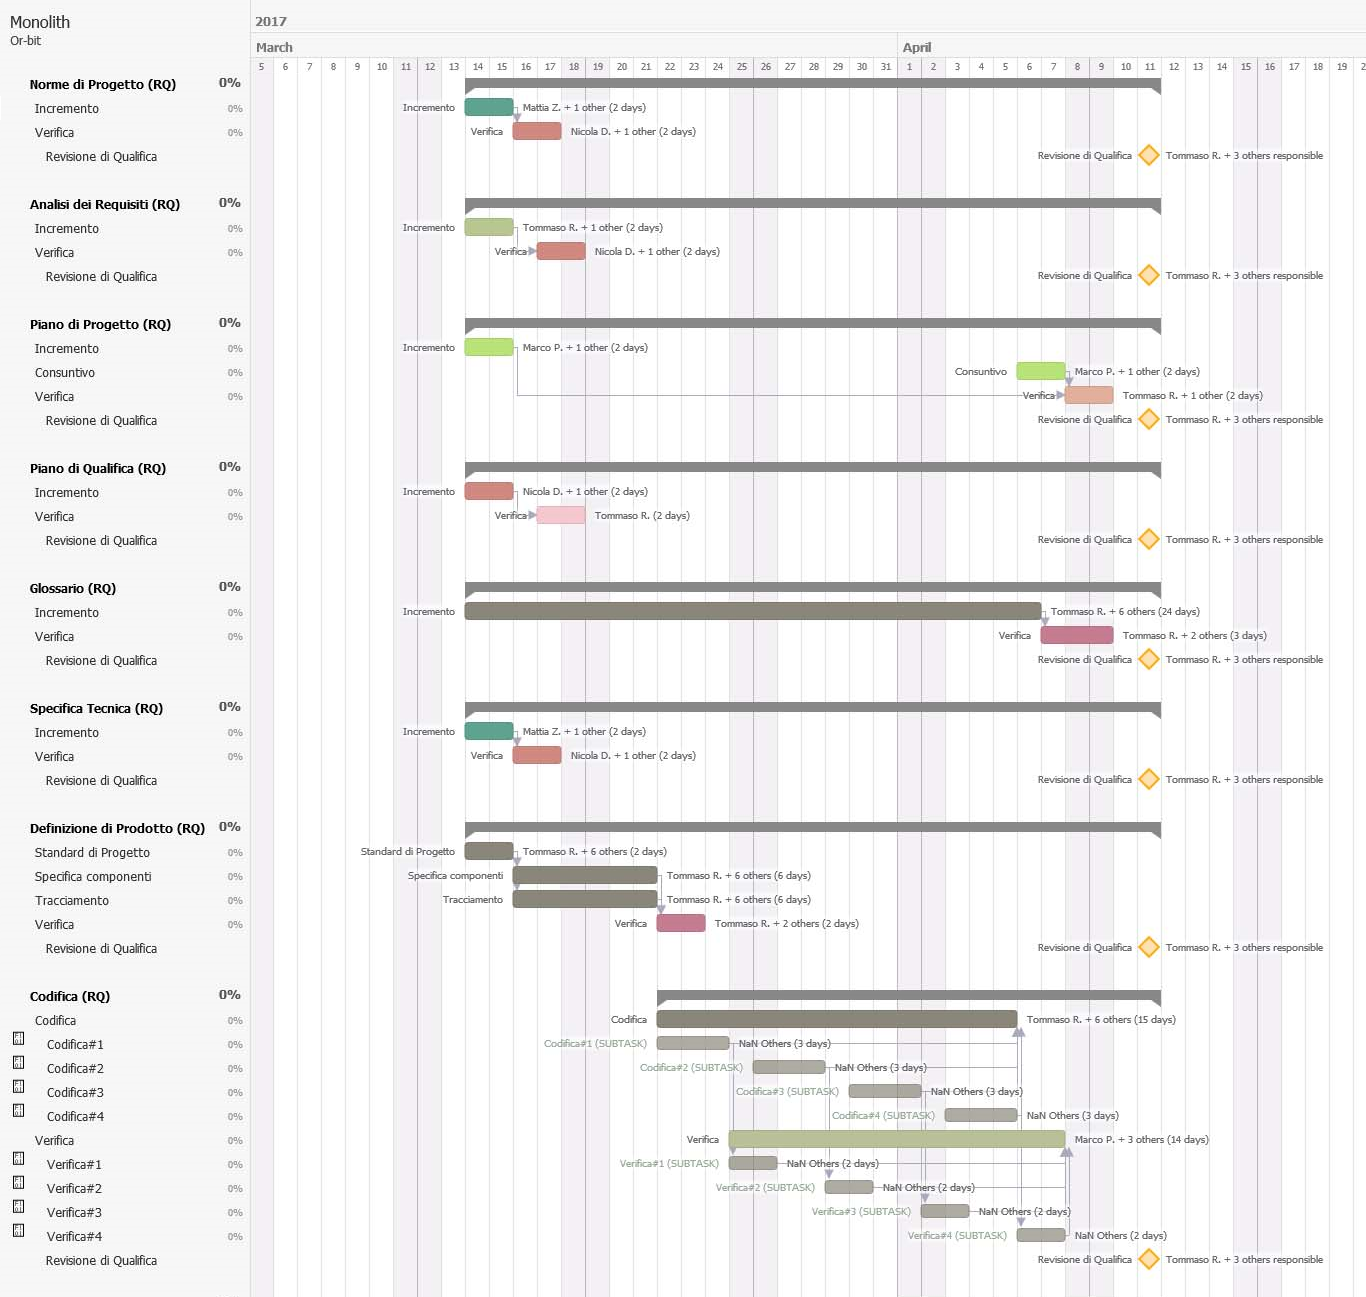
\includegraphics[width=15cm]{gantt/Gantt_RQ2.png}
	\caption{Diagramma di Gantt, periodo di \PD{} e \Cod{}}
\end{figure}

\subsubsection{Ripartizione ore}
\bgroup
\egroup

\subsection{\VV{}}
\textbf{Periodo:} da 19-04-2017 a 08-05-2017. \\
Il periodo di \VV{} è il periodo finale del progetto, prevede la verifica di tutto il sistema realizzato e la conformità con i requisiti del capitolato.
Nel periodo di Analisi i ruoli maggiormente coinvolti sono \Programmatore{}, \Progettista{}, \Responsabile{}, \Amministratore{} e \Verificatore{}.
\subsubsection{Gantt attività}
\begin{figure}[H]
	\centering
	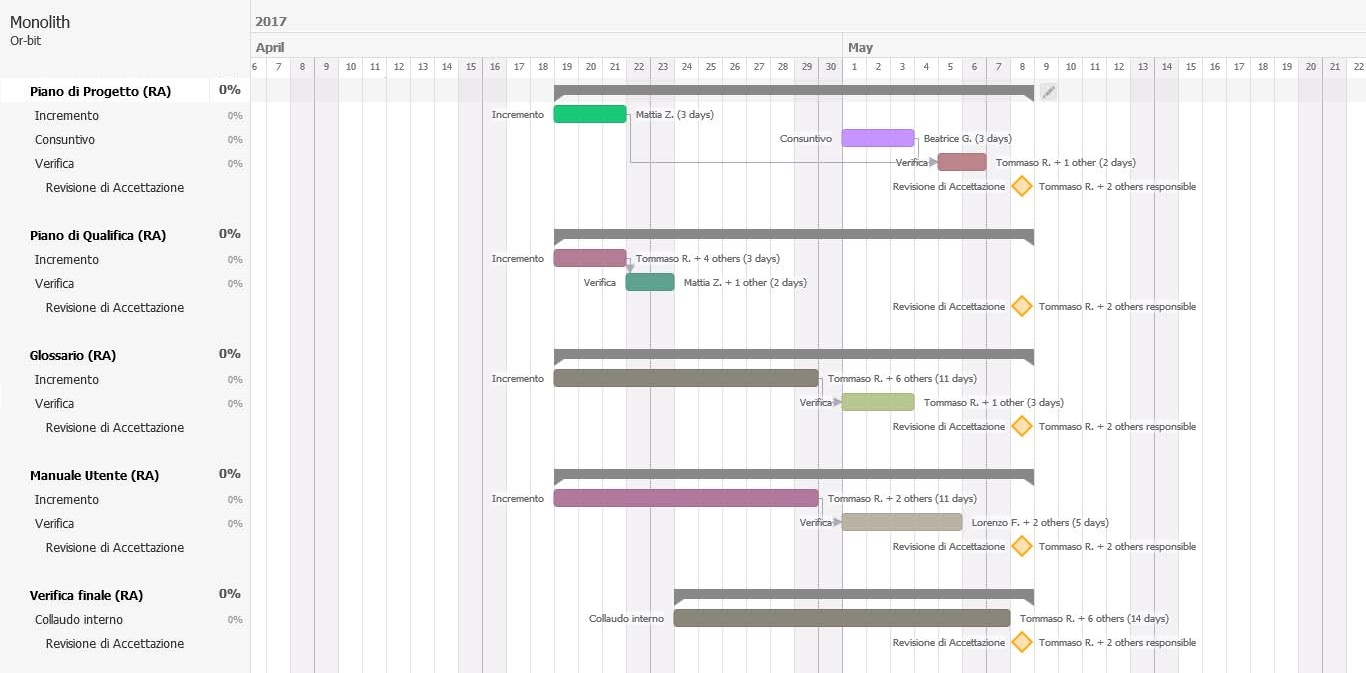
\includegraphics[width=15cm]{gantt/Gantt_RA2.png}
	\caption{Diagramma di Gantt, periodo di \VV{}}
\end{figure}

\subsubsection{Ripartizione ore}
\bgroup
\egroup

